\subsubsection{ARcore}
\begin{table}[H]
	\centering
	\begin{tabular}{|c|c|}
		\hline
		\multicolumn{2}{|c|}{Especificaciones de prueba}   \\ \hline
		\textbf{DISPOSITIVO}              & Moto G6 XT1925 \\ \hline
		\textbf{FECHA}                    & 2018/08/25     \\ \hline
		\textbf{VERSIÓN DE SCENEFORM SDK} & V1.4.0         \\ \hline
		\textbf{VERSIÓN DE ARCORE SDK}    & V1.4.0         \\ \hline
		\textbf{VERSIÓN DE ANDROID}       & V8.0.0 (Oreo)  \\ \hline
	\end{tabular}
	\captionsetup{justification=centering}
	\caption{Especificaciones de prueba Arcore en Moto G6}
\end{table}

\textbf{Posición cardinal} \par
El objeto virtual se pudo apreciar con claridad desde los cuatro puntos cardinales y la vista superior. El ángulo de visualización del objeto al mover la cámara cambiaba a la perfección, dando una buena percepción de realismo.

%%IMAGENES DE PUNTOS CARDINALES
\begin{figure}[!htbp]
	\begin{minipage}{0.48\textwidth}
	\centering
		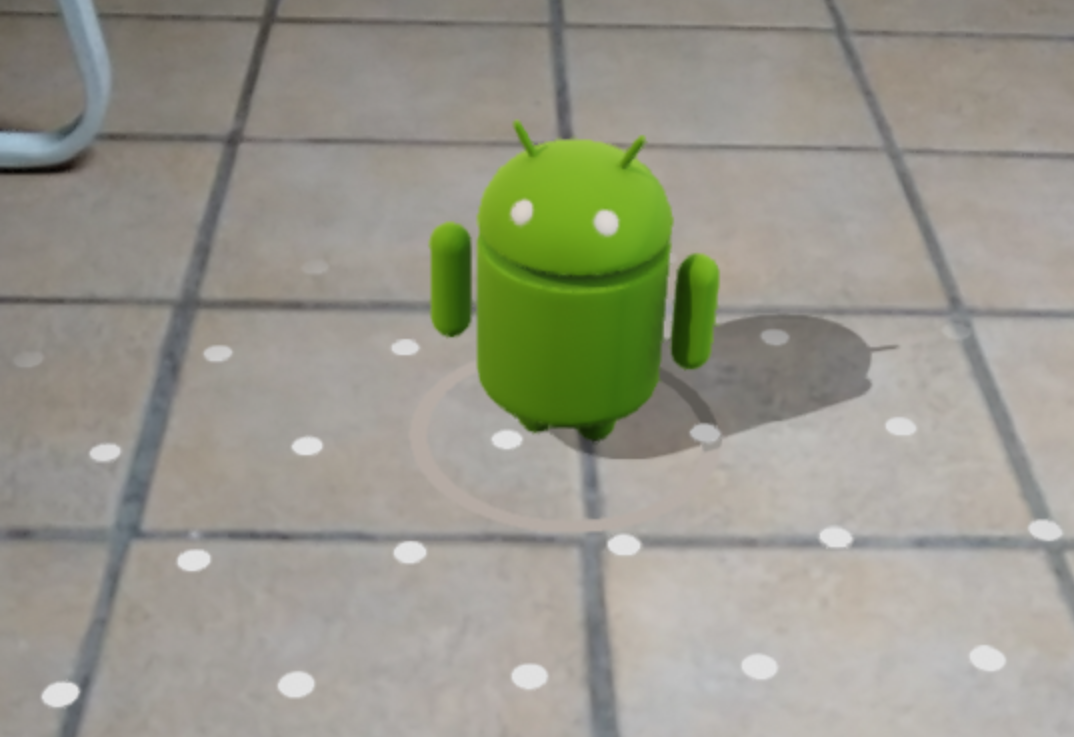
\includegraphics[width=8cm]{desarrollo/secciones/pruebas/motog6/img/NORTE.png}
		\caption{Posición Norte}
		\label{fig:motog6norte}
	\end{minipage}\hfill
	\begin{minipage}{0.48\textwidth}
	\centering
	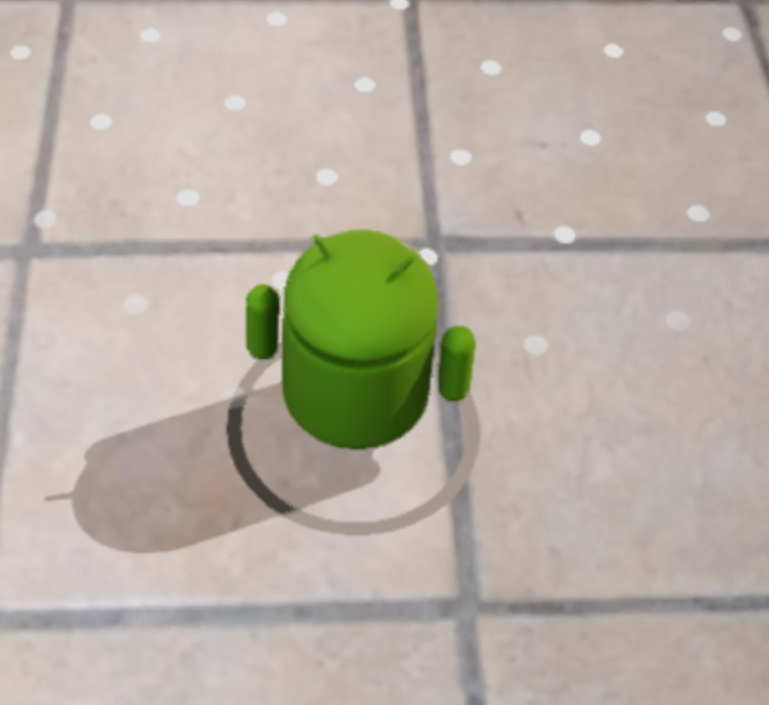
\includegraphics[width=8cm]{desarrollo/secciones/pruebas/motog6/img/SUR.png}
	\caption{Posición Sur}
	\label{fig:motog6sur}
	\end{minipage}\hfill
\end{figure}

\begin{figure}[!htbp]
	\begin{minipage}{0.48\textwidth}
		\centering
		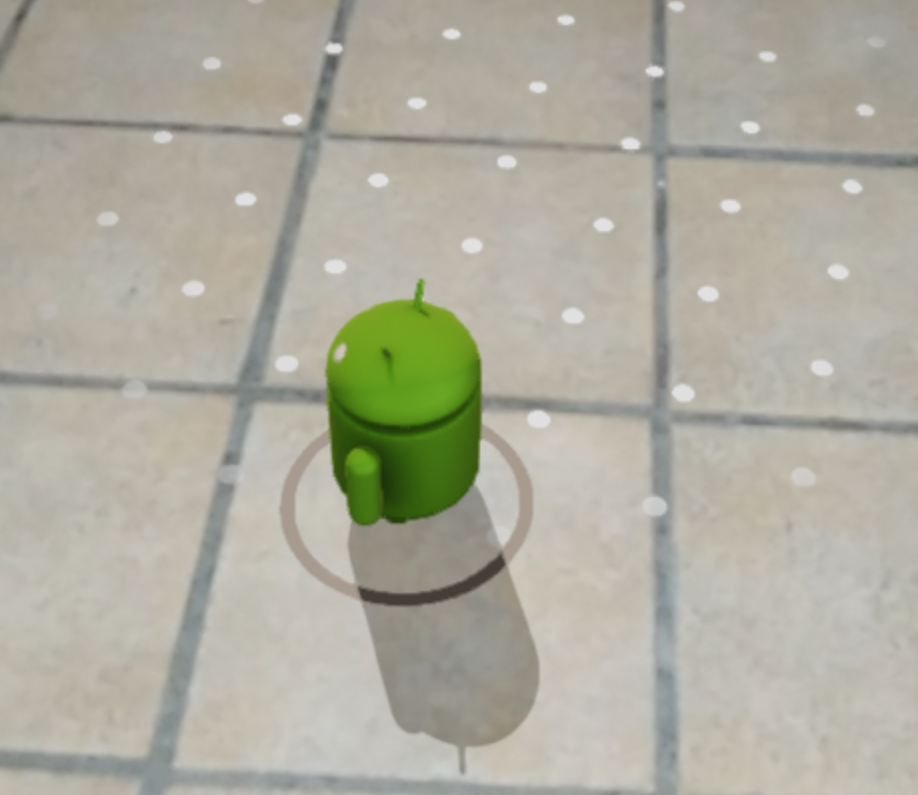
\includegraphics[width=8cm]{desarrollo/secciones/pruebas/motog6/img/ESTE.png}
		\caption{Posición Este}
		\label{fig:motog6norte}
	\end{minipage}\hfill
	\begin{minipage}{0.48\textwidth}
		\centering
		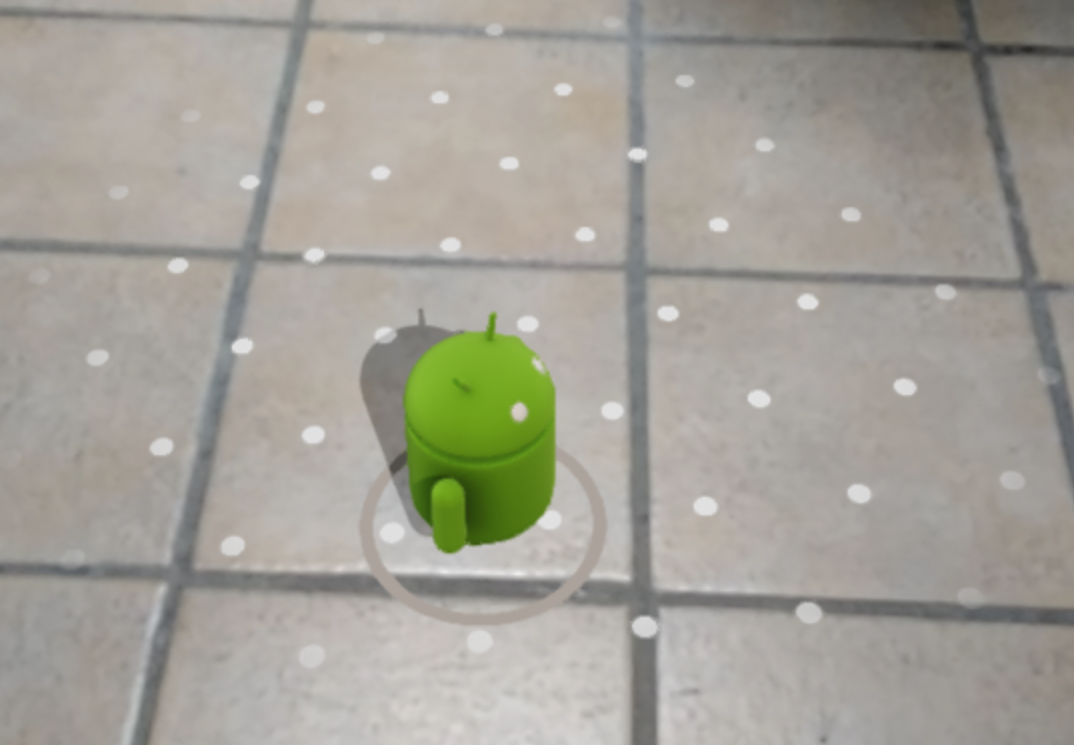
\includegraphics[width=8cm]{desarrollo/secciones/pruebas/motog6/img/OESTE.png}
		\caption{Posición Oeste}
		\label{fig:motog6oeste}
	\end{minipage}\hfill
\end{figure}

\textbf{Tamaño relativo} \par
Al acercar o alejar la cámara el objeto virtual variaba su tamaño de forma adecuada, como si el objeto realmente estuviera en la posición donde fue superpuesto.


\begin{figure}[!htbp]
	\begin{minipage}{0.48\textwidth}
		\centering
		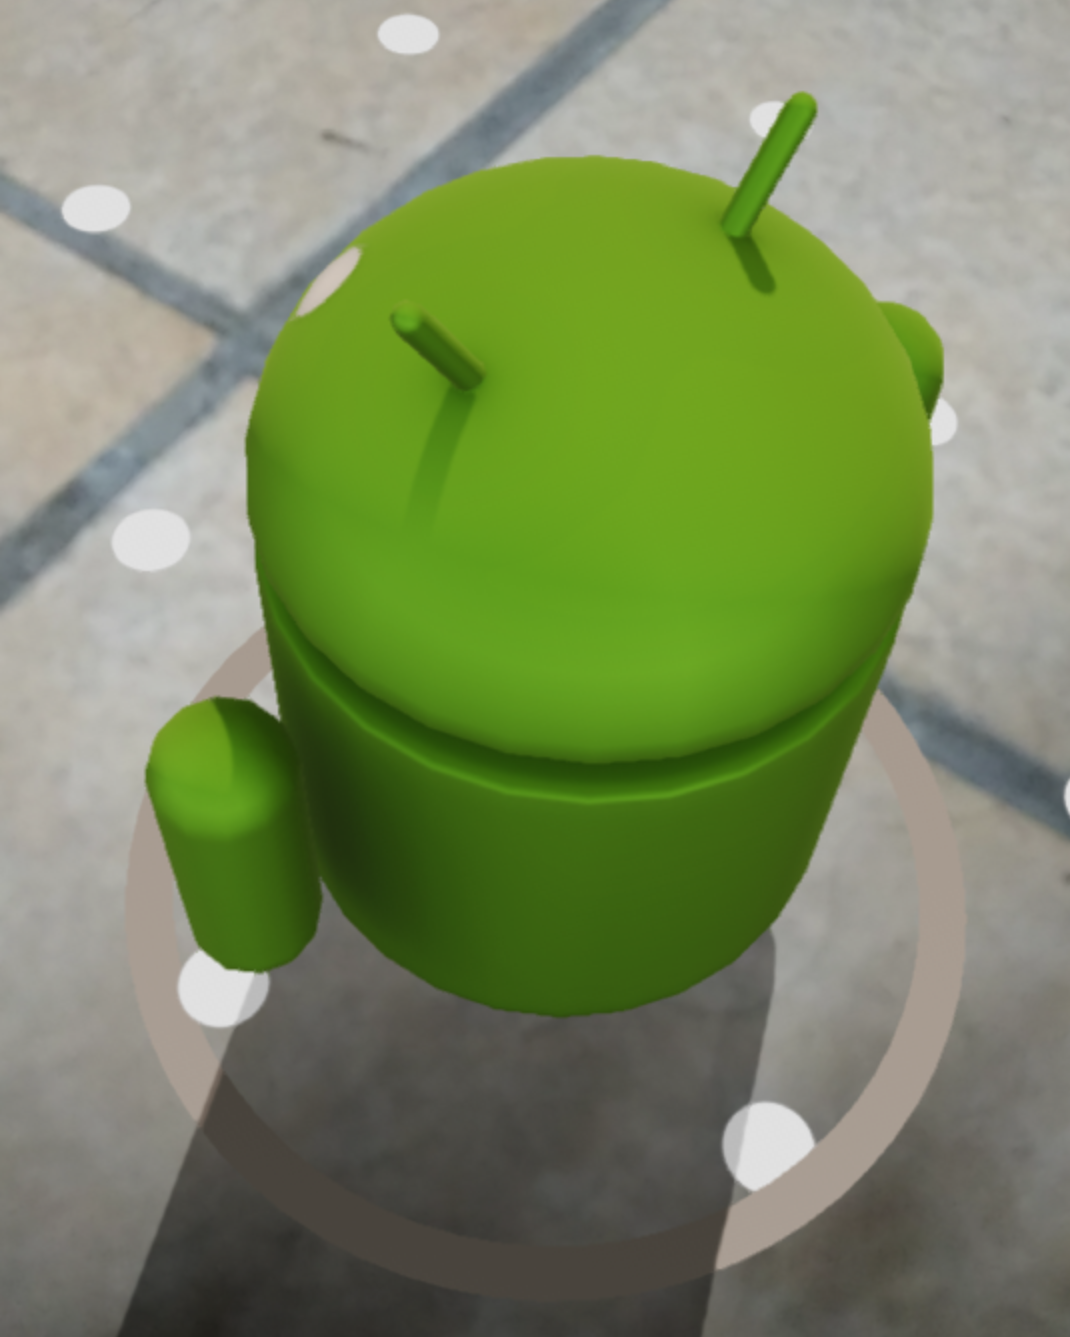
\includegraphics[width=8cm]{desarrollo/secciones/pruebas/motog6/img/CERCA.png}
		\caption{Objeto visto de cerca}
		\label{fig:motog6cerca}
	\end{minipage}\hfill
	\begin{minipage}{0.48\textwidth}
		\centering
		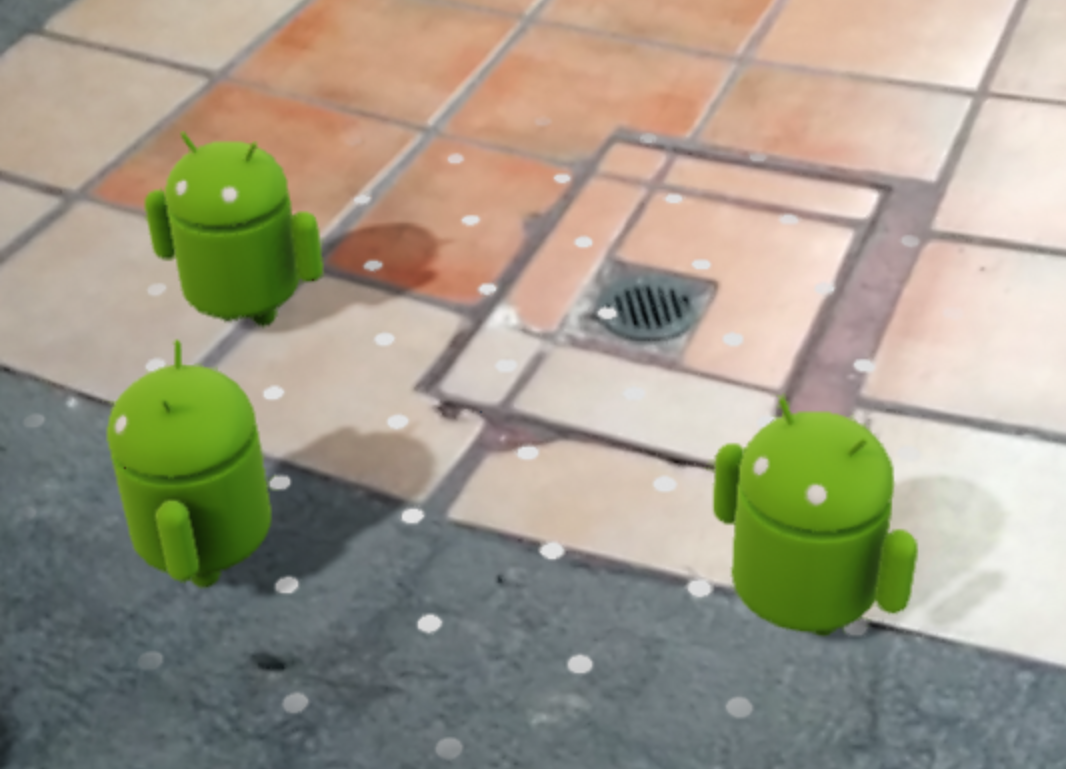
\includegraphics[width=8cm]{desarrollo/secciones/pruebas/motog6/img/LUZALTA.png}
		\caption{Luz alta}
		\label{fig:motog6lalta}
	\end{minipage}\hfill
\end{figure}

\textbf{Luminosidad} \par
Al poner el objeto virtual en entornos con diferente cantidad de luz, la cantidad de luz en el objeto virtual también variaba. En un entorno con ausencia casi total de luz el objeto apenas era perceptible, mientras que en un entorno con bastante luz, el objeto se veía altamente iluminado.

\begin{figure}[!htbp]
	\begin{minipage}{0.48\textwidth}
		\centering
		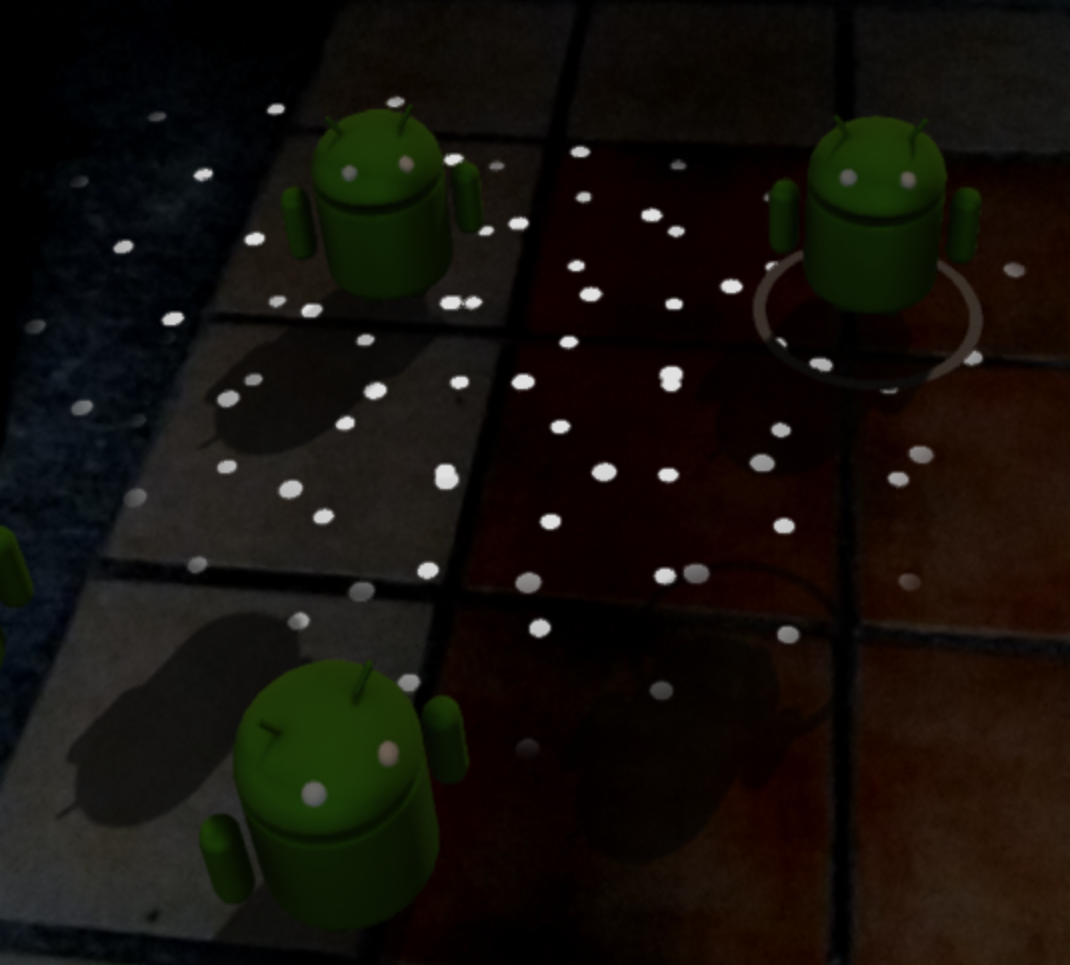
\includegraphics[width=8cm]{desarrollo/secciones/pruebas/motog6/img/LUZBAJA.png}
		\caption{Luz baja}
		\label{fig:motog6lbaja}
	\end{minipage}\hfill
	\begin{minipage}{0.48\textwidth}
		\centering
		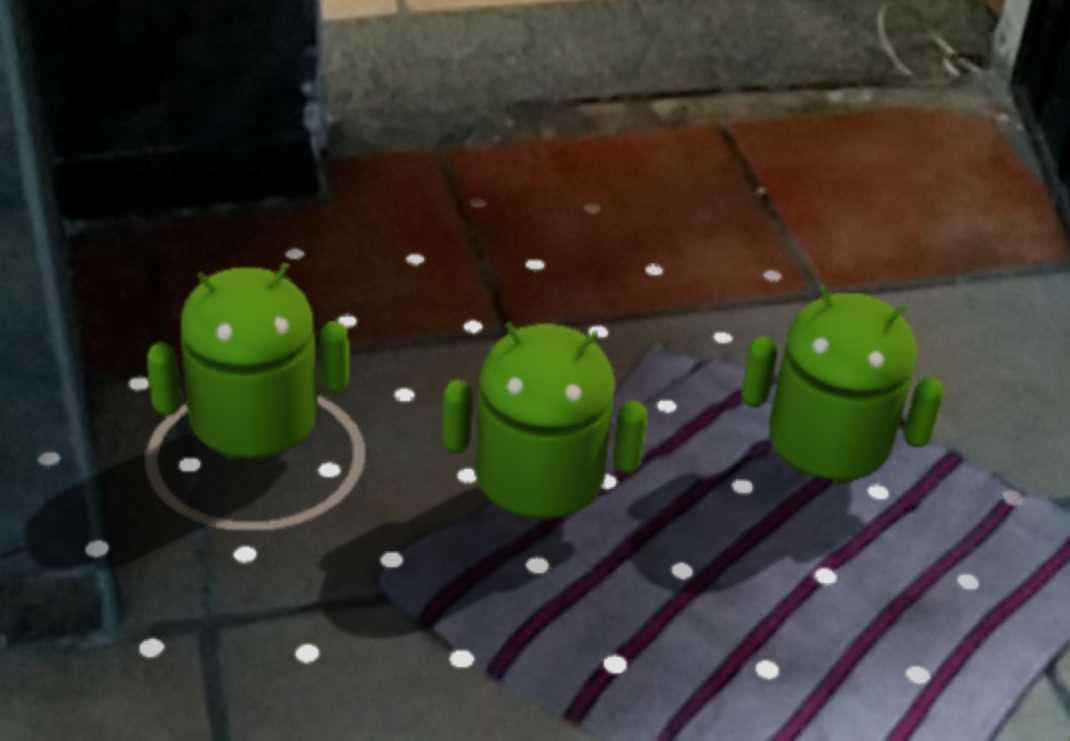
\includegraphics[width=8cm]{desarrollo/secciones/pruebas/motog6/img/LUZMEDIA.png}
		\caption{Luz media}
		\label{fig:motog6lmedia}
	\end{minipage}\hfill
\end{figure}

\textbf{Superficie} \par
Se probó posicionar el objeto virtual en cuatro superficies: concreto gris, concreto blanco, azulejo y vidrio.\par
Concreto gris.- El objeto se pudo posicionar a la perfección.\par
Concreto blanca.- El objeto no se pudo posicionar. La maya de puntos ni si quiera era detectada en ésta superficie debido a la ausencia de texturas.\par
Azulejo.- El objeto se pudo posicionar a la perfección.\par
Vidrio.- El objeto no pudo ser posicionado en ésta superficie debido a las propiedades reflejantes que posee.\par

\begin{figure}[!htbp]
	\begin{minipage}{0.48\textwidth}
		\centering
		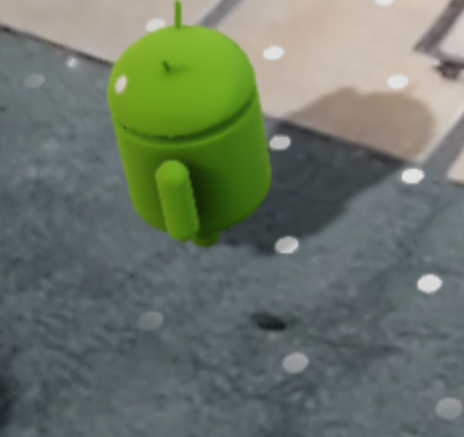
\includegraphics[width=8cm]{desarrollo/secciones/pruebas/motog6/img/CONCRETO.png}
		\caption{Objeto colocado en concreto}
		\label{fig:motog6concreto}
	\end{minipage}\hfill
	\begin{minipage}{0.48\textwidth}
		\centering
		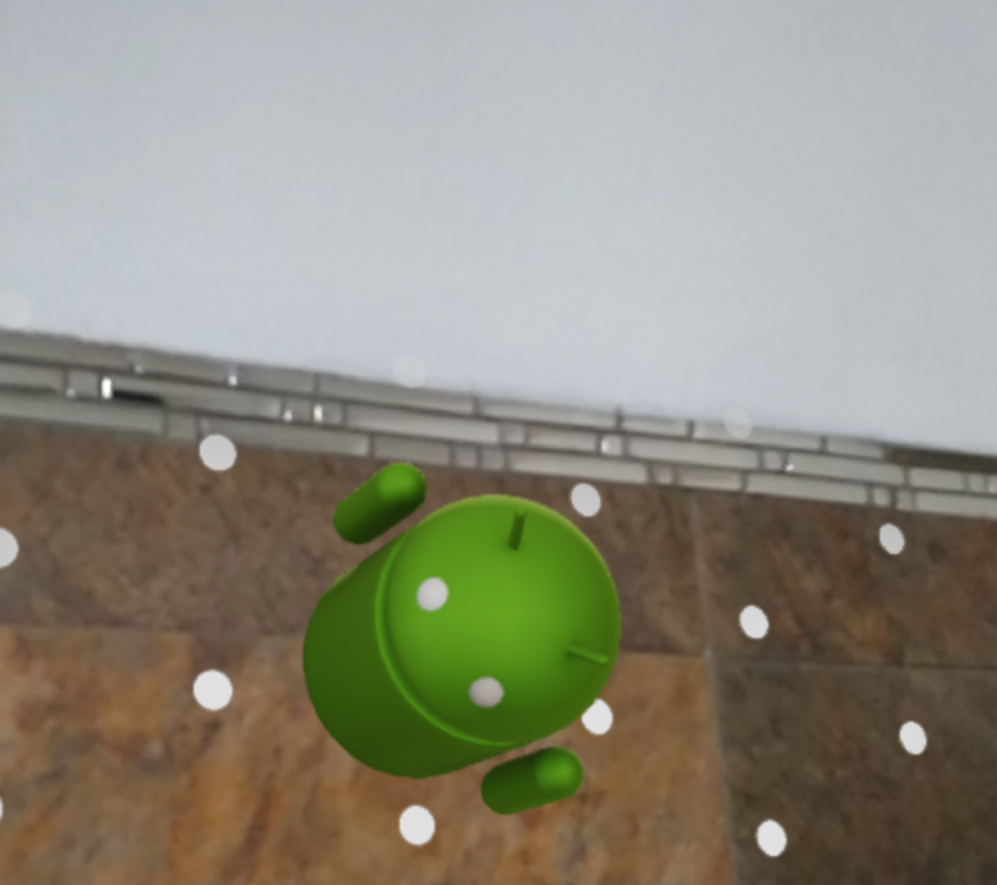
\includegraphics[width=8cm]{desarrollo/secciones/pruebas/motog6/img/SUPBLANCA.png}
		\caption{Objeto colocado en superficie blanca}
		\label{fig:motog6supblanca}
	\end{minipage}\hfill
\end{figure}

\begin{figure}[H]
	\begin{minipage}{0.48\textwidth}
		\centering
		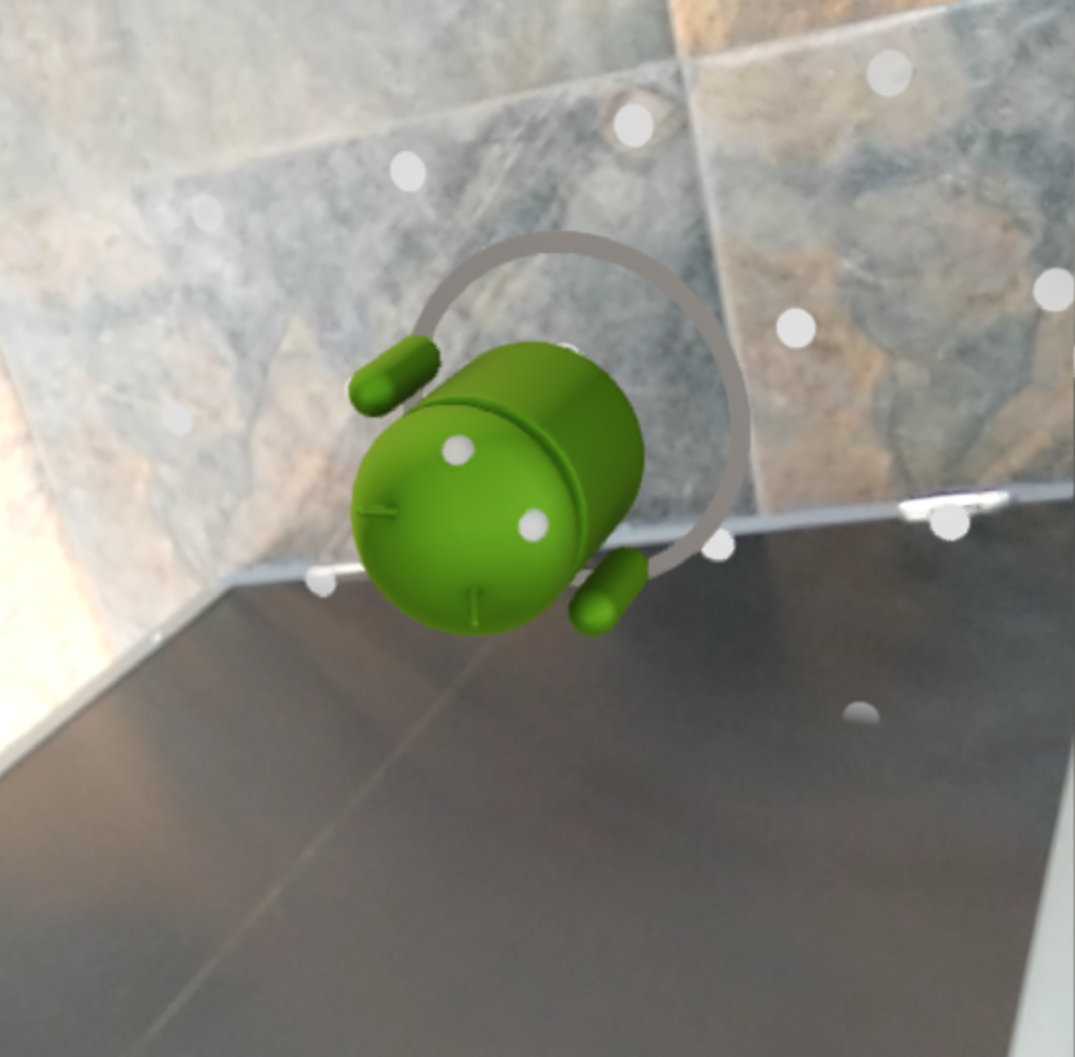
\includegraphics[width=8cm]{desarrollo/secciones/pruebas/motog6/img/SUPERFICIENEGRA.png}
		\caption{Malla de puntos no detectada en superficie negra}
		\label{fig:motog6supnegra}
	\end{minipage}\hfill
	\begin{minipage}{0.48\textwidth}
		\centering
		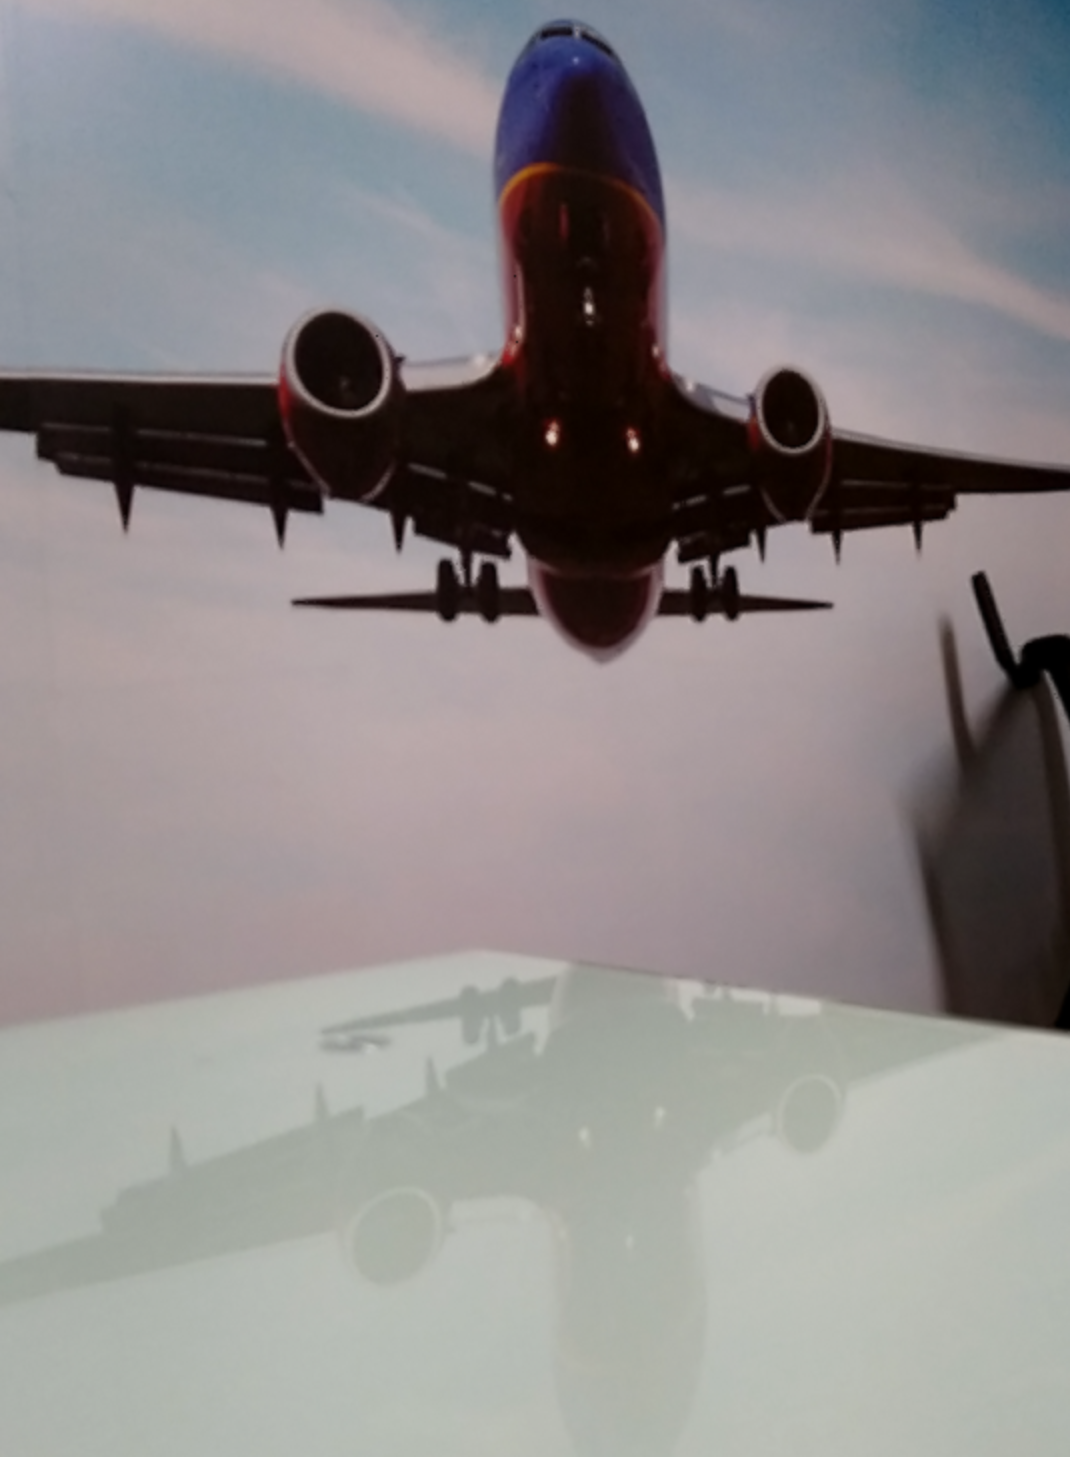
\includegraphics[width=6cm]{desarrollo/secciones/pruebas/motog6/img/VIDRIO.png}
		\caption{Malla de puntos no detectada en vidrio}
		\label{fig:motog6vidrio}
	\end{minipage}\hfill
\end{figure}

\textbf{\\Memoria de objetos} \par
Tras perder el enfoque de la cámara, al volverlo a tener, todos los objetos virtuales se volvieron a mostrar en el entorno virtual en la misma posición en la que habían sido puestos.

\textbf{Capacidad máxima de objetos} \par
Se colocaron 100 objetos virtuales en escena sin que la aplicación perdiera rendimiento. Todo funcionaba con total fluidez.

\begin{figure}[H]
	\begin{minipage}{0.48\textwidth}
		\centering
		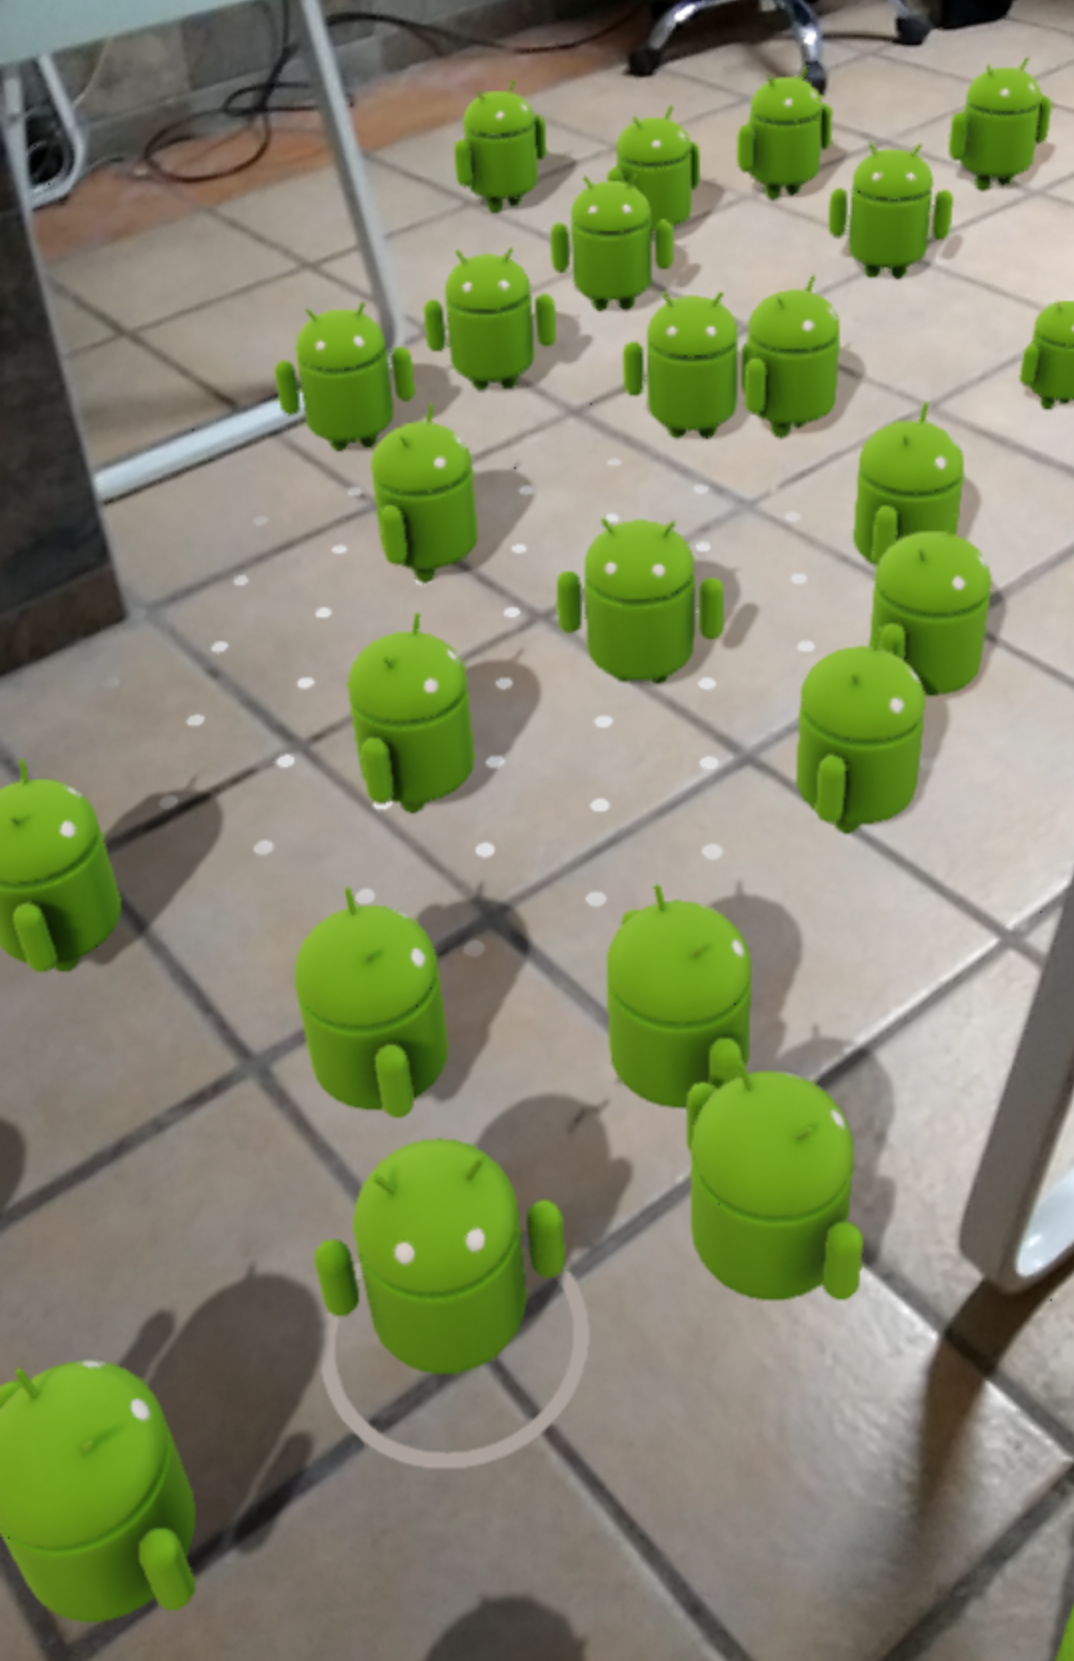
\includegraphics[width=5cm]{desarrollo/secciones/pruebas/motog6/img/CANTIDAD.png}
		\caption{Gran cantidad de objetos en escena}
		\label{fig:motog6escena}
	\end{minipage}\hfill
	\begin{minipage}{0.48\textwidth}
		
		\centering
		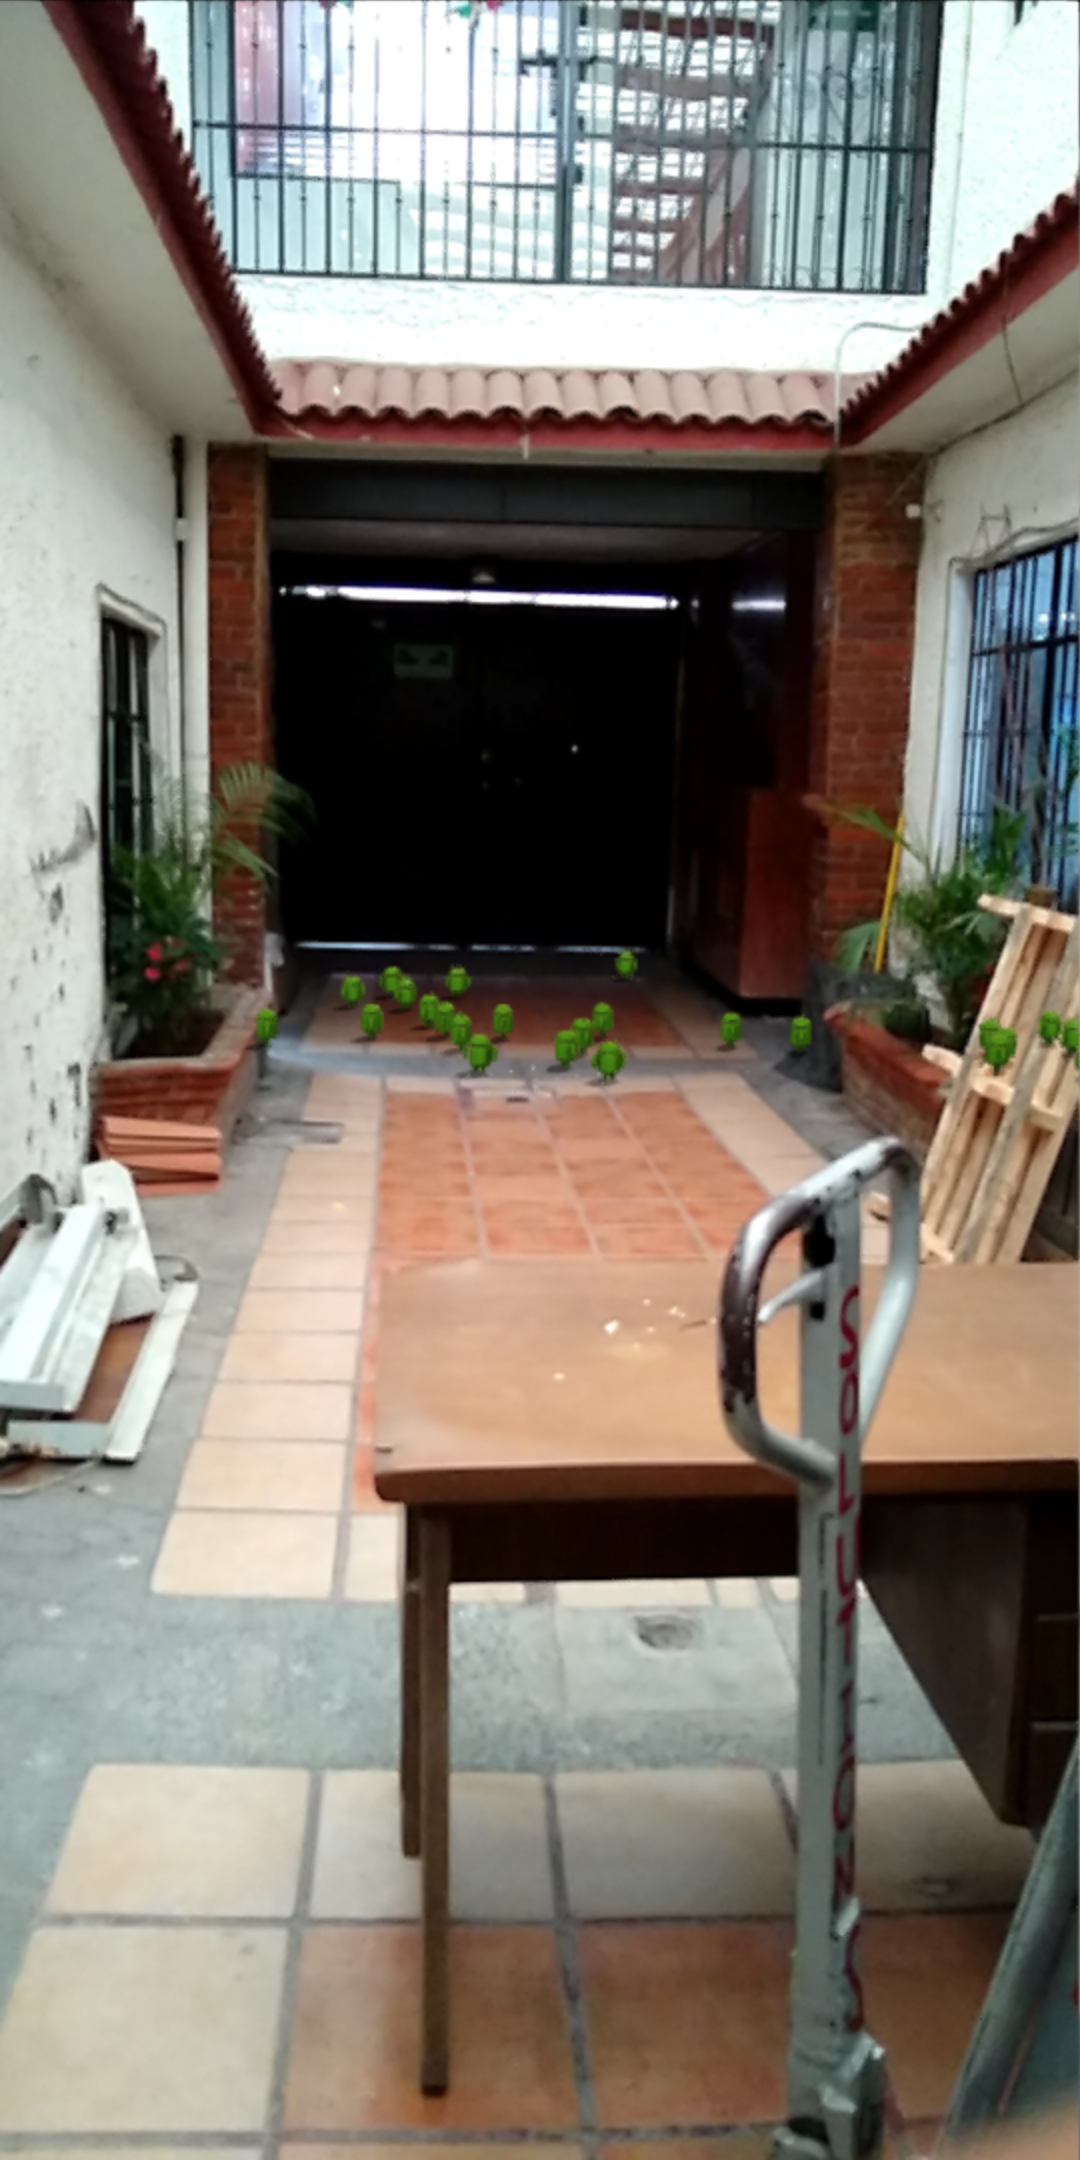
\includegraphics[width=5cm]{desarrollo/secciones/pruebas/motog6/img/DISTANCIA.png}
		\caption{Objetos puestos a gran distancia}
		\label{fig:motog6edistancia}
	\end{minipage}\hfill
\end{figure}

\textbf{Distancia} \par
Se colocó un objeto, después la cámara fue alejada hasta una distancia de \textbf{11.22m.} A esa distancia los objetos comenzaron a verse pixeleados, además comenzaron a desaparecer y reaparecer de forma intermitente.

